\chapter{Дизайн и реализация}

В предыдущем разделе были рассмотрены структуры данных используемые файловыми
системами ZFS и Btrfs - ZFS использует хеш-таблицы, а Btrfs B+ деревья. Этот
раздел посвящен дизайну и реализации файловой системы использующей вариацию
структуры данных известную как LSM-дерево.

Текущая реализация файловой системы находится в состоянии proof-of-concept, т.
е. многие существенные для файловой системы функции еще не реализованы:
\begin{itemize}
  \item согласно спецификации POSIX если файл был удален, пока хотя бы один из
        процессов файловой системы держит файловый дескриптор ссылающийся на
        этот файл, то файл все еще должен быть доступен этому процессу - такое
        поведение часто называют отложенным удалением, и оно не поддерживается
        в текущей реализации;
  \item другая важная функциональность файловой системы заключается в
        отслеживании свободного и занятого места на диске, однако организация
        хранения этой информации является довольно сложной задачей, которая не
        решена в текущей версии кода, т. е. файловая система может работать
        только в режиме append-only.
\end{itemize}

\section{LSM-деревья}

Подход LSM-деревьев был предложен в статье~\cite{LSM}. Основная идея лежащая в
основе LSM-деревьев заключается в том, что изменения индексной структуры
накапливаются в памяти, после чего большими порциями выписываются на диск в
отсортированном порядке и по возможности последовательно. Дополнительно к
основному алгоритму в~\cite{BLSM} описываются несколько оптимизаций и
модификаций, которые позволяют сделать LSM-деревья более дружелюбными по
отношению к запросам на чтение. Далее в этом разделе описывается вариация
LSM-деревьев использованная в данный момент в реализации myfs.


\subsection{Структура LSM-деревьев}

LSM-дерево состоит из нескольких уровней, который далее будут обозначаться как
$C_i$, где $i$ - это целое неотрицательное число, которое обозначает номер
уровня. Уровни $C_0$ и $C_1$ - это уровни которые хранятся в памяти. Все
остальные уровни ($C_i$, где $i > 1$) хранятся на диске. Количество уровней
фиксировано и никогда не изменяется\footnote{Побочный эффект такого ограничения
это логарифмическая сложность поиска, однако основной причиной этого ограничения
является не алгоритмическая сложность, а простота реализации.}. Каждый уровень
представляет из себя упорядоченный словарь.


\subsubsection{Операции над LSM-деревом}

Все операции обновления индекса (вставка и удаление ключей) всегда выполняются
над уровнем $C_0$. Если операция вставки не вызывает вопросов, то операция
удаления ключа требует пояснений так как LSM-дерево состоит из нескольких
словарей. Операция удаления ключа заключается в добавлении этого ключа со
специальным маркером, который будет обозначать, что этот ключ удален. В
последствии ключи с таким маркером будут удалены из дерева.

По мере работы над LSM-деревом ключи будут переходить от уровней с меньшими
номерами в уровни с большими номерами посредством выполнения операции слияния.
Таким образом для поиска ключа в LSM-дереве необходимо выполнить поиск
последовательно на каждом уровне начиная с 0 до тех пор пока ключ не будет
найден. Если при этом у ключа присутствует маркер-признак того, что ключ был
удален, то значит в LSM-дереве искомый ключ отсутствует. При выполнении запросов
возвращающих ключи в некотором диапазоне придется просмотреть все уровни и
объединить результаты из каждого из этих уровней.


\subsubsection{Перенос данных из памяти на диск}

По мере выполнения операций вставки и удаления словарь $c_0$ в памяти может
стать очень большим, и в какой момент может потребоваться сохранить данные из
памяти на диск. Эта операция называется flush и она выполняется в два этапа:
\begin{itemize}
  \item $C_0$ переносится в $C_1$, а словарь $C_0$ инициализируется пустым
        множеством пар;
  \item над словарями $C_1$ и $C_2$ выполняется операция слияния, которая
        создает новый словарь.
\end{itemize}

Перенос из $C_0$ в $C_1$ требуется для того, чтобы не блокировать операции
записи на время сохранения данных на диск. Перенос $C_0$ в $C_1$ фактически
сводится к подмене нескольких указателей в памяти, т. е. выполняется довольно
быстро. После этого можно продолжать выполнение операций вставки/удаления над
новым пусты $C_0$, в то время как $C_1$ остается неизменным во время выполнения
операции слияния.

Кроме того, разделение на два этапа требуется для эффективного создания
контрольной точки файловой системы на диске с минимальными задержками для
пользователей. Подробнее о реализации создании контрольной точки и использовании
flush рассказывается в разделе~\ref{sec:commit}.


\subsection{Слияние деревьев}

Ключевой в работе LSM-деревьев является операция слияния подробнее рассмотренная
ниже. Как уже упоминалось выше слияние выполняется, если $C_0$ в памяти стал
слишком большим. Однако, если поддерживать только 3 уровня $C_0$,
вспомогательный $C_1$ и $C_2$, то по мере роста размера индекса выполнение
операции слияния будет занимать слишком много времени, так как слияние требует
последовательного прохода по обеим сливаемым последовательностям.

Действительно, если $C_2$ будет расти неограниченно, то его размер начнет
доминировать время выполнения слияния. Фактически в этом случае на каждое
слияние $C_1$ и $C_2$ придется вычитывать и перезаписывать большую часть
индекса. Чтобы этого избежать этого в myfs размер $C_2$ ограничивается так,
чтобы слияние можно было выполнять сравнительно быстро.


\subsubsection{Ограничения на размеры уровней}
\label{sec:lsmlev}

В текущей реализации используется ограничение в 2Mb на размер $C_2$. При
превышении ограничения уровень $C_2$ будет слит с уровнем $C_3$. Всего уровней
6: $C_0$ и $C_1$ в памяти, $C_2$ - $C_5$ на диске. Размеры уровней на диске
образуют геометрическую прогрессию с основанием 4. Т. е. размер уровня $C_3$
ограничен 8 Mb, размер уровня $C_4$ 32 Mb, а последний уровень $C_5$ не имеет
ограничения так как его уже нескем сливать.

Количество деревьев было выбрано из следующих соображений. В типичной домашней
файловой системе может содержаться порядка миллиона файлов и каталогов. Простой
скрипт на языке Python:

\begin{lstlisting}[language = Python]
#!/usr/bin/env python

import os

total_len, total_size, nitems, nfiles = 0, 0, 0, 0
for path, dirs, files in os.walk('/'):
    to_remove = []

    for name in dirs:
        fullname = os.path.join(path, name)
        # exclude pseudo filesystems
        if fullname in ('/sys', '/proc', '/media'):
            to_remove.append(name)
            continue
        total_len += len(name)

    for name in to_remove:
        dirs.remove(name)

    for name in files:
        fullname = os.path.join(path, name)
        total_len += len(name)
        if not os.path.islink(fullname) and os.path.isfile(fullname):
            total_size += os.stat(fullname).st_size
            nfiles += 1

    nitems += len(dirs) + len(files)

print 'entries: {}, avg size: {}, avg len {}'.format(nitems,
    total_size / nfiles, total_len / nitems)
\end{lstlisting}
Запущенный на компьютере автора демонстрирует, что суммарное количество записей
во всех каталогах (включая символьные и жесткие ссылки) чуть более полумиллиона,
а средний размер имени всего 15 байт. Служебная информация с учетом имени,
которая хранится для каждой такой записи в файловой системе myfs занимает
порядка 54 байт, таким образом 6-и уровней достаточно чтобы сохранить всю
информацию о структуре каталогов и иметь некоторый запас.


\subsubsection{Операция слияния}

Операция слияния выполняется над двумя последовательными словарями $C_i$ и
$C_{i+1}$ в результате создавая новый словарь $C'_{i+1}$ на диске, содержащий
элементы $C_i$ и $C_{i+1}$. После завершения слияния словари $C_i$ и $C_{i+1}$
больше не требуются, словарь $C_{i+1}$ подменяется новым словарем $С'_{i+1}$,
а словарь $C_i$ подменяется пустым словарем.

Так как все словари поддерживают данные в упорядоченном виде\footnote{Можно
также отсортировать пары ключ/значения из словаря перед слиянием}, то слияние
требует одного прохода по каждому словарю и выполняется за линейное от
количества пар время подобно операции слияния в алгоритме сортировки слиянием.

При слиянии однако требуется специальная обработка одинаковых ключей. Например,
в ситуации, когда $C_i$ и $C_{i+1}$ содержат один и тот же ключ, но ключ из
$C_i$ содержит маркер-признак удаленного ключа, то в результирующий словарь
должен попасть только ключ с этим маркером. Таким образом в случае совпадения
ключей из $C_i$ и $C_{i+1}$ в результирующий словарь $C'_{i+1}$ попадает только
более новый ключ из $C_i$.

Более того, если $C_{i+1}$ является последним используемым уровнем в дереве и
ключ содержит маркер-признак удаленного ключа, то мы можем не добавлять его в
результирующее дерево. Таким образом дойдя до последнего уровня в дереве ключ
с маркером удаляется из LSM-дерева физически.


\subsection{Словарь в памяти}

В качестве словаря в памяти (для уровней $C_0$ и $C_1$) используется lock-free
реализация структуры данных известной как SkipList~\cite{SKIP}.


\subsubsection{Интерфейс словаря в памяти}

Словарь в памяти должен поддерживать интерфейс описываемый структурой
myfs\_mtree из inc/lsm/lsm.h:
\begin{lstlisting}
struct myfs_mtree {
    int (*insert)(struct myfs_mtree *, const struct myfs_key *,
                  const struct myfs_value *);

    int (*lookup)(struct myfs_mtree *, struct myfs_query *);
    int (*range)(struct myfs_mtree *, struct myfs_query *);
    int (*scan)(struct myfs_mtree *, struct myfs_query *);

    size_t (*size)(const struct myfs_mtree *);
};
\end{lstlisting}

В этой структуре есть только одна операция модификации - insert. Благодаря тому,
что данные реально не удаляются, вместо этого вставляются ключи со специальным
маркером не требуется поддерживать специально операцию удаления, что упрощает
также реализацию lock-free алгоритма, так как не требуется заботиться о
безопасном освобождении памяти при удалении ключей\footnote{Все еще нужно уметь
освобождать дерево целиком после того, как его содержимое было сохранено на
диск. О том, как это организовано рассказывается дальше.}.

Далее идут три операции поиска:
\begin{itemize}
    \item lookup - точечный поиск одного значения удовлетовряющего некоторому
          предикату, согласующемуся с порядком хранения элементов в словаре;
    \item range - запрос поиска всех значений входящих в некоторый диапазон
          заданный некоторым предикатом, согласующимся с порядком хранения
          элементов в словаре;
    \item scan - поиск всех элементов, удовлетворяющих некоторому произвольному
          предикату.
\end{itemize}

Во всех случаях предикат задается как в виде структуры myfs\_query определенной
в inc/types.h:
\begin{lstlisting}
struct myfs_query {
    int (*cmp)(struct myfs_query *, const struct myfs_key *);
    int (*emit)(struct myfs_query *, const struct myfs_key *,
                const struct myfs_value *);
};
\end{lstlisting}

В этой структуре поле cmp проверяет удовлетворяет ли значение предикату. Эта
функция должна возвращать 0, если переданный ключ удовлетворяет предикату, -1
если переданный ключ меньше искомого и 1 если больше. Функция emit вызывается
для каждой пары ключ значение, которые удовлетворяют заданному предикату.

Последняя часть интерфейса словаря в памяти - это функция size. Функция должна
возвращать примерное количество записей в словаре. Эта функция используется
чтобы проверить необходимость сохранения словаря на диск.


\subsubsection{Разрешение коллизий в словаре в памяти}

При работе со словарем в памяти один и тот же ключ может быть добавлен несколько
раз. Например, чтобы удалить ключ из LSM-дерева этот ключ добавляется в дерево
со специальным маркером. В такой ситуации, вместо того чтобы изменять элемент
уже хранящийся в SkipList-е в словарь добавляется новый элемент. Изменение уже
хранящегося элемента не желательно так как он может в данный момент
использоваться, например, при конкурентом запросе на поиск. Эту проблему можно
преодолеть используя техники безопасного освобождения памяти, такие как RCU или
Hazrd Pointer, но в целях простоты реализации было решено использовать другой
подход.

Используемый подход заключается в добавлении к элементу уникального
идентификатора. Причем идентификаторы по мере работы с SkipList-ом монотонно
возрастают. Элементы с большим идентификатором, т. е. более новые, считаются
меньше элементов с меньшим идентификатором, если ключи элементов равны. Таким
образом благодаря идентификатору всегда можно понять какой элемент является
последней версией.


\subsection{Словарь на диске}

Словарь на диске создается при выполнении операции слияния. После того как
словарь был создан он никогда не изменяется, но может быть в будущем заменен
новым словарем.

В качестве словаря на диске используется сильноветвистое идеально
сбалансированное дерево поиска подобное B+ дереву. Выбор структуры обусловлен
двумя факторами:
\begin{itemize}
  \item в таком дереве поиска легко искать значения по ключу не читая его в
        память целиком, в отличие, например, от классических SSTable,
        часто используемых при реализации LSM-деревьев;
  \item создавать такое дерево из отсортированного потока элементов не сильно
        сложнее чем SSTable, так как достаточно всего лишь одного прохода по
        отсортированной последовательности элементов.
\end{itemize}


\subsubsection{Интерфейс словаря на диске}

Словарь на диске поддерживает операции похожие на операции словаря в памяти за
исключением операции scan. Кроме того, так как словарь на диске никогда не
изменяется, после того как был создан, то дополнительно реализован интерфейс
итераторов. Изменение интерфейса обусловлено несколькими обстоятельствами:
\begin{itemize}
  \item полный просмотр словаря на диске требуется только при выполнении
        операции слияния и использовать итератор для этого удобнее так как
        необходимо сканировать два словаря одновременно;
  \item при выполнении запросов на диапазоне требуется просмотр каждого словаря
        на диске, используя итераторы легко реализовать запросы на диапазоне без
        загрузки всего диапазона целиком в память;
  \item реализовать scan, если потребуется, легко используя итератор, а вот
        обратное сделать тяжелее, если предполагать, что словарь на диске может
        не поместиться в память.
\end{itemize}

\subsubsection{Структура словаря на диске}

Каждый узел дерева на диске начинается со структуры \_\_myfs\_ctree\_node\_sb
описанной в файле inc/lsm/ctree.h:
\begin{lstlisting}
struct __myfs_ctree_node_sb {
        le32_t items;
        le32_t size;
} __attribute__((packed));
\end{lstlisting}

Структра хранит число элементов и количество байт, которые занимает узел дерева.
Далее следую собственно элементы, хранящиеся в узле дерева, перед каждым
элементом хранится структура \_\_myfs\_ctree\_item:
\begin{lstlisting}
struct __myfs_ctree_item {
        le32_t key_size;
        le32_t value_size;
} __attribute__((packed));
\end{lstlisting}
Каждый элемент состоит из пары ключ и значение, размеры ключа и значения в
байтах и хранятся в этой структуре.

В листьях дерева хранятся ключи и значения добавленные в дерево, во внутренних
узлах хранятся только ключ, а вместо настоящих значений хранятся указатели на
дочерние листы дерева (файл inc/types.h):
\begin{lstlisting}
struct __myfs_ptr {
    le64_t offs;
    le64_t size;
    le64_t csum;
} __attribute__((packed));
\end{lstlisting}

В указателе на каждый узел дерева хранится 64-битная контрольная сумма, чтобы
иметь возможность проверять целостность узла. Указатель на корень дерева, а
также некоторая дополнительная информация сохраняются в структуре
\_\_myfs\_ctree\_sb:
\begin{lstlisting}
struct __myfs_ctree_sb {
    struct __myfs_ptr root;
    le32_t size;
    le32_t hight;
} __attribute__((packed));
\end{lstlisting}


\subsubsection{Построение словаря на диске}

Как отмечалось выше построение словаря на диске может быть выполнено за один
проход по отсортированной последовательности элементов. Во время построения
словаря на диске алгоритм поддерживает данные на нескольких уровнях. Новые
элементы добавляются на 0-ой уровень. Этот уровень соответствует листьям дерева
поиска. Когда нулевой уровень заполняется он выписывается на диск как узел
дерева, при этом на уровень 1 добавляется новый элемент состоящий из наибольшего
ключа выписанного узла дерева и указателя на этот узел (структура
\_\_myfs\_ptr). По мере заполнения уровня 1 данные этого уровня также будут
выписаны на диск в качестве узла дерева и новый элемент будет добавлен на
уровень 2. Этот процесс продолжается пока не будут обработаны все элементы
входной последовательности.

При выписывании дерева контролируется его ветвистость. В текущей реализации
узел выписывается только если количество элементов в нем не менее 16 либо
если больше нет элементов для добавления в дерево. 


\subsection{Выбор ветвистости дерева}

В текущей реализации ветвистость дерева определяется следующим образом:
\begin{itemize}
  \item узел с менее чем 16 ключами выписывается только в том случае, если не
        осталось элементов для добавления в дерево;
  \item если в узле уже есть 16 элемента и размер узла выровненный на ближайшую
        сверху границу страницы позволяет добавлять ключи, то ключи добавляются
        в узел.
\end{itemize}

Такой подход выбран по следующим соображениям. Все операции ввода/вывода
осуществляются блоку кратному размеру страницы файловой системы\footnote{Размер
страницы определяется при форматировании, по-умолчанию она равен 4096 байтам.},
таким образом, если в узле еще осталось достаточно места до ближайшей сверху
границы страницы, то его нужно использовать, в противном случае оно будет
потрачено зря.

Минимальная ветвистость дерева определялась на основании следующих соображений.
При тестировании было показано, что время поиска в дереве на диске доминируется
временем подсчета хеша узла\footnote{Хеш используется для проверки
целостности.}. Для этого был проведен следующий эксперимент:
\begin{enumerate}
  \item создается дерево на диске с $10^8$ элементами;
  \item производится $10^8$ случайных поисков в дереве;
\end{enumerate}

\begin{figure}[h]
  \centering
  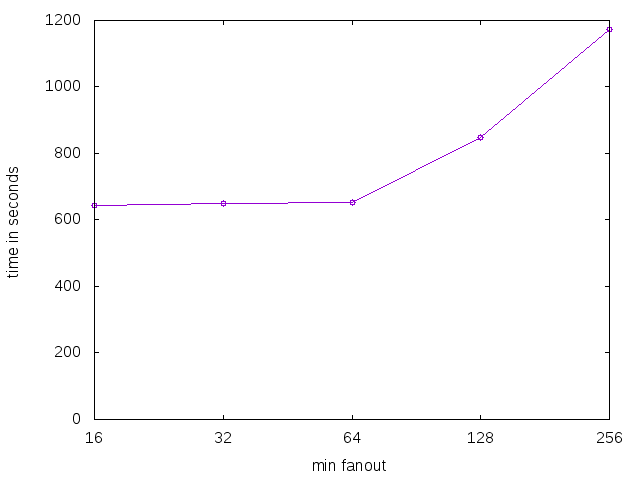
\includegraphics[width=.8\textwidth]{impl/fanout.png}
  \caption{Время работы в зависимости от ветвистости узла}
  \label{pic:fanout}
\end{figure}

Эксперимент повторяется три раза и выбирается время минимальной из попыток. Этот
эксперимент повторялся для разных значений минимальной ветвистости: 16, 32, 64,
128, 256. Результаты эксперимента вы можете увидеть на рисунке~\ref{pic:fanout}.
Как вы можете увидеть, при небольших значениях минимальной ветвистости
результаты отличаются незначительно, но при увеличении ветвистости время
выполнения начинает резко возрастать.

\begin{table}[h]
  \centering
  \begin{subfigure}{.5\textwidth}
    \begin{tabular}{ r l }
        overhead & symbol \\ \hline
        23.29\% & [ctree] XXH64 \\
        21.48\% & [ctree] myfs\_ctree\_it\_find \\
        14.51\% & [kernel] copy\_user\_enhanced\_fast\_string \\
        5.35\%  & [kernel] \_\_radix\_tree\_lookup \\
        3.27\%  & [kernel] find\_get\_entry \\
        2.77\%  & [libc] \_int\_malloc \\
        2.52\%  & [libc] \_int\_free \\
        2.36\%  & [kernel] generic\_file\_read\_iter \\
        2.33\%  & [ctree] ctree\_query\_cmp \\
        1.53\%  & [kernel] entry\_SYSCALL\_64 \\
    \end{tabular}
    \caption{ветвистость 16}
  \end{subfigure}
  \begin{subfigure}{.5\textwidth}
    \begin{tabular}{ r l }
        overhead & symbol \\ \hline
        28.61\% & [ctree] XXH64 \\
        24.20\% & [ctree] myfs\_ctree\_it\_find \\
        17.74\% & [kernel] copy\_user\_enhanced\_fast\_string \\
        4.02\%  & [kernel] \_\_radix\_tree\_lookup \\
        3.18\%  & [kernel] find\_get\_entry \\
        2.61\%  & [kernel] generic\_file\_read\_iter \\
        1.67\%  & [libc] \_int\_malloc \\
        1.42\%  & [libc] \_int\_free \\
        1.40\%  & [ctree] ctree\_query\_cmp \\
        1.11\%  & [libc] \_\_memcmp\_sse4\_1 \\
        0.98\%  & [kernel] copy\_page\_to\_iter \\
        0.93\%  & [kernel] entry\_SYSCALL\_64 \\
    \end{tabular}
    \caption{ветвистость 256}
  \end{subfigure}
  \caption{Результаты профилирования утилитой perf}
  \label{tbl:prof}
\end{table}

Это можно объяснить следующим образом, при небольших значениях минимальной
ветвистости количество элементов в узле определяется размером страницы, однако,
когда элементы перестают помещаться в одну страницу результаты начинают
ухудшаться, так как возрастает время на подсчет хеша прочитанного узла. Это
подтверждается результатами профилирования в таблице~\ref{tbl:prof}. Как вы
можете заметить большая часть времени работы приходится на функцию XXH64,
которая занимается вычислением хеша.

Таким образом при точечных запросах имеет смысл использовать минимально
возможные узлы дерева, чтобы сократить время на подсчет хешей узлов. Однако
ограничивать ветвистость исключительно размером страницы нельзя, так как при
больших размерах элементов с ростом высоты дерева будет ухудшаться
алгоритмическая сложность поиска в таком дереве. Поэтому в качестве минимальной
ветвистости было выбрано число 16 - минимальное из протестированных значений.

Затрат на подсчет хешей прочитанных узлов можно избежать поддерживая кеш узлов.
Так как даже при случайных запросах некоторые узлы будут использоваться довольно
часто\footnote{Например, корень дерева используется всеми запросами, узлы
близкие к корню также могут использоваться довольно часто.}. Однако в текущей
реализации кеширование узлов дерева не реализовано.


\subsection{Синхронизация доступа к LSM-дереву}

Доступ к LSM-дереву контролируется несколькими блокировками:
\begin{itemize}
  \item read/write блокировка mtlock для словарей в памяти;
  \item read/write блокировка sblock для словарей на диске;
  \item блокировка mtx для защиты при выполнении слияния.
\end{itemize}

Read/write блокировка для словарей в памяти используется следующим образом. Все
операции модификации и поиска в словаре в памяти перед чтением указателя на
словарь захватывают блокировку на чтение. После завершения операции блокировка
отпускается. Так как словарь в памяти использует lock-free реализацию
SkipList-а, то никакой посторонней синхронизации эти операции не требуют.

Однако, при слиянии словаря в памяти со словарем на диске нам необходимо
дождаться пока словарь стабилизируется, т. е. все операции вставки будут
завершены, поэтому манипуляции с указателями на словари в памяти выполняются с
mtlock захваченной на запись. Вместо read/write блокировки можно было бы
воспользоваться одним из механизмов безопасного освобождения памяти, но опять же
в целях простоты реализации было принято решение использовать именно блокировку.

Read/write блокировка для словарей на диске используется аналогичным к mtlock
образом. Все операции поиска в дереве, а также операция чтения указателей на
корень дерева захватывают блокировку на чтение. По завершению операции
блокировка отпускается. Однако в отличие от mtlock держать блокировку в течение
всего времени выполнения операции не обязательно, так как в текущей реализации
занятое однажды место никогда не переиспользуется.

Наконец блокировка mtx используется чтобы защитить массив флагов намерения
слияния. Чтобы избежать ситуации когда один и тот же словарь используется в двух
конкурирующих операциях слияния перед выполнением операции необходимо захватить
блокировку mtx, подождать пока флаг намерения соответствующий нужному словарю
обнулиться, после чего выставить этот флаг тем самым показав намерение
использовать данный словарь при выполнении операции слияния. По завершении
операции слияния флаг необходимо обнулить.

\section{Реализация файловой системы}

Имея на руках готовую реализацию словаря в виде LSM-дерева можно использовать
его в качестве индексной структуры для файловой системы. Более того так как
LSM-деревья не перезаписывают словари на диске, а вместо этого создают новые, то
по крайней мере индексы файловой системы автоматически будут COW.

В myfs в силу ее простоты и небогатой функциональности достаточно всего двух
LSM-деревьев (см. структуру myfs в файле inc/myfs.h):
\begin{itemize}
  \item inode\_map - хранит так называемые индексные узлы;
  \item dentry\_map - хранит дерево каталогов.
\end{itemize}
Структура элементов и назначение каждого из этих LSM-деревьев в деталях
обсуждается далее в этом разделе.


\subsection{Библиотека FUSE}

Filesystem in Userspace (далее FUSE) - это библиотека и драйвер ядра ОС, который
позволяет реализовать драйвер файловой системы совершенно полностью в
пространстве пользователя. Использование FUSE упрощает разработку файловой
системы в ряде аспектов:
\begin{itemize}
  \item для пространства пользователя доступно множество средств диагностики и
        отладки приложений;
  \item разрабатывать файловую систему можно на любом удобном языке при условии,
        что есть возможность подключения библиотеки в языку.
\end{itemize}

При этом разработанная файловая система может использоваться наравне с файловыми
системами включенными в ядро ОС. Благодаря этому можно без изменений
использовать бенчмарки и тесты существующие для файловых систем.

Однако использование FUSE также может отразиться на производительности в связи
с тем, что каждый запрос к файловой системе сначала поступает в ядро, потом из
ядра через FUSE передается в пространство пользователя драйверу файловой
системы. Ответ на каждый запрос аналогичным образом передается назад
пользователю. Кроме того, если файловая система пользуется интерфейсом
ввода/вывода предоставляемым ядром ОС, то это еще дополнительные расходы на
системные вызовы, которых не было бы у драйвера ядра.


\subsubsection{Интерфейс файловой системы}

Существует два вида интерфейсов, которые должен реализовать драйвер файловой
системы чтобы использовать FUSE. Эти интерфейсы условно называются
низкоуровневым и высокоуровневым. Высокоуровневый интерфейс в основном состоит
из набора функций похожих на стандартные для Unix операций работы с файлами и
каталогами:
\begin{lstlisting}
struct fuse_operations {
    ...
    int (*mkdir) (const char *, mode_t);
    int (*unlink) (const char *);
    int (*rmdir) (const char *);
    int (*symlink) (const char *, const char *);
    int (*rename) (const char *, const char *, unsigned int);
    int (*link) (const char *, const char *);
    ...
    int (*open) (const char *, struct fuse_file_info *);
    int (*read) (const char *, char *, size_t, off_t,
                 struct fuse_file_info *);
    int (*write) (const char *, const char *, size_t, off_t,
                  struct fuse_file_info *);
    ...
    int (*opendir) (const char *, struct fuse_file_info *);
    int (*readdir) (const char *, void *, fuse_fill_dir_t, off_t,
                    struct fuse_file_info *, enum fuse_readdir_flags);
    ...
};
\end{lstlisting}

За исключением некоторого отличия в количестве и именах операций низкоуровневый
интерфейс отличается от высокуровневого типом идентификатора файла/каталога. В
высокоуровневом интерфейсе используется путь, в то время к в низкоуровневом
интерфейсе для этого используется номер индексного узла (далее просто inode):
\begin{lstlisting}
struct fuse_lowlevel_ops {
    ...
    void (*lookup) (fuse_req_t req, fuse_ino_t parent, const char *name);
    ...
    void (*mknod) (fuse_req_t req, fuse_ino_t parent, const char *name,
                   mode_t mode, dev_t rdev);
    void (*mkdir) (fuse_req_t req, fuse_ino_t parent, const char *name,
                   mode_t mode);
    void (*unlink) (fuse_req_t req, fuse_ino_t parent, const char *name);
    void (*rmdir) (fuse_req_t req, fuse_ino_t parent, const char *name);
    void (*symlink) (fuse_req_t req, const char *link, fuse_ino_t parent,
                     const char *name);
    void (*rename) (fuse_req_t req, fuse_ino_t parent, const char *name,
                    fuse_ino_t newparent, const char *newname,
                    unsigned int flags);
    void (*link) (fuse_req_t req, fuse_ino_t ino, fuse_ino_t newparent,
                  const char *newname);
    void (*read) (fuse_req_t req, fuse_ino_t ino, size_t size, off_t off,
                  struct fuse_file_info *fi);
    void (*write) (fuse_req_t req, fuse_ino_t ino, const char *buf,
                   size_t size, off_t off, struct fuse_file_info *fi);
    ...
    void (*readdir) (fuse_req_t req, fuse_ino_t ino, size_t size, off_t off,
                     struct fuse_file_info *fi);
    ...
};
\end{lstlisting}

Так как работать с номерами индексных узлов несколько проще чем с полными
именами, то в реализации принято решение использовать низкоуровневый интерфейс.


\subsection{Хранение дерева каталогов}

Для хранения дерева каталогов в myfs используется LSM-дерево dentry\_map. В
качестве ключа в дереве выступает структура \_\_myfs\_dentry\_key (см. файл
inc/dentry.h):
\begin{lstlisting}
struct __myfs_dentry_key {
    le64_t parent;
    le32_t hash;
    le32_t size;
    char name[1];
} __attribute__((packed));
\end{lstlisting}

Ключ хранит номер inode каталога, которому принадлежит эта запись - parent. А
также хеш имени, длина имени (без учета завершающего нулевого символа) и само
имя записи в каталоге. Все эти поля участвую в сравнении.

В качестве значения используется структура \_\_myfs\_dentry\_value:
\begin{lstlisting}
    le64_t inode;
    le32_t type;
\end{lstlisting}
В значение входят аттрибуты которые не участвуют в сравнении: номер inode
файла/каталога, на который ссылается запись, и тип (файл или каталог).

Таким образом информация о дереве каталогов файловой системы внутри dentry\_map
кодируется в виде ссылки на родителя.


\subsubsection{Поиск файла/каталога в каталоге по имени}

Чтобы уметь обходить дерево каталогов ОС от файловой системе требуется
реализация операции поиска по имени внутри заданного каталога. В структуре
fuse\_lowlevel\_ops за эту операцию отвечает поле lookup.

В случае dentry\_map эта операция реализуется как обычный точечный поиск. В
качестве ключа используется номер inode каталога и имя (хеш, длина имени и само
имя).


\subsubsection{Итерация по каталогу}

Для реализации таких команд как ls, ОС предоставляет интерфейс, который
позволяет перечислять содержимое каталога. В структуре fuse\_lowlevel\_ops
за итерацию по каталогу отвечает поле readdir:
\begin{lstlisting}
    void (*readdir) (fuse_req_t req, fuse_ino_t ino, size_t size, off_t off,
                     struct fuse_file_info *fi);
\end{lstlisting}

В качестве параметров операция принимает номер inode каталога, содержимое
которого необходимо перечислить, а также смещение (off). Однако смещение не смотря на
название не обязано обозначать смещение внутри каталога. Это может быть любое
целое число, которое каким-то образом сообщит драйверу файловой системы с какого
места в каталоге нужно начать перечисление. Изначально смещение должно быть
равно 0. Все значения отличные от 0, это значения возвращенные файловой
системой, соответственно, она должна знать как именно их использовать.

Все записи в dentry\_map принадлежащие одному каталогу упорядочены по хешу.
Таким образом можно использовать хеш в качестве смещения внутри каталога. Таким
образом myfs и использует хеш имени в текущей реализации. Однако стоит отметить,
что в редких случаях коллизий хешей и неудачном стечении обстоятельств
последовательное применение операции readdir чтобы прочитать содержимое каталога
может привести к тому, что некоторые записи в каталоге "потеряются". Такой же
проблемой обладает, например, файловая система ext4.

Существуют способы исправить эту проблему, однако на данный момент они не
реализованы и поэтому будут рассмотрены в разделе~\ref{sec:todo}.


\subsection{Словарь inode-ов}

Индексный узел или inode - это некоторая структура файловой системы, котрая
хранит информацию о файле или каталоге. Информация, которую хранит inode, может
включать в себя:
\begin{itemize}
  \item тип (файл, каталог или какая-то другая сущность файловой системы);
  \item владелец файла (пользователь, группа пользователя);
  \item права доступа к файлу (кто может его читать/писать/исполнять);
  \item различные временные метки (дата создания, дата модификации, дата
        доступа);
  \item различные атрибуты связанные с размером (каков логический размер файла
        каталога, сколько места занято на диске);
  \item информация о местах диска, где размещено содержимое файла/каталога.
\end{itemize}

Чтобы получить примерное представление об информации, которую хранит inode можно
обратиться к структуре stat определенной в стандарте POSIX\footnote{Данная
версия взята не из стандарта POSIX, а из описания man 2 stat согласующегося со
спецификацией POSIX.}:
\begin{lstlisting}
struct stat {
    dev_t     st_dev;         /* ID of device containing file */
    ino_t     st_ino;         /* inode number */
    mode_t    st_mode;        /* protection */
    nlink_t   st_nlink;       /* number of hard links */
    uid_t     st_uid;         /* user ID of owner */
    gid_t     st_gid;         /* group ID of owner */
    dev_t     st_rdev;        /* device ID (if special file) */
    off_t     st_size;        /* total size, in bytes */
    blksize_t st_blksize;     /* blocksize for filesystem I/O */
    blkcnt_t  st_blocks;      /* number of 512B blocks allocated */

    /* Since Linux 2.6, the kernel supports nanosecond
       precision for the following timestamp fields.
       For the details before Linux 2.6, see NOTES. */
     struct timespec st_atim;  /* time of last access */
     struct timespec st_mtim;  /* time of last modification */
     struct timespec st_ctim;  /* time of last status change */

     #define st_atime st_atim.tv_sec      /* Backward compatibility */
     #define st_mtime st_mtim.tv_sec
     #define st_ctime st_ctim.tv_sec
};
\end{lstlisting}


В myfs для хранения inode-ов используется отдельное LSM-дерево inode\_map.
Ключом в этом дереве является структура \_\_myfs\_inode\_key (см. файл
inc/inode.h):
\begin{lstlisting}
struct __myfs_inode_key {
    le64_t inode;
} __attribute__((packed));
\end{lstlisting}

А в качестве значения выступает структура \_\_myfs\_inode\_value:
\begin{lstlisting}
struct __myfs_bmap_entry {
    le64_t disk_offs;
    le64_t file_offs;
} __attribute__((packed));

struct __myfs_bmap {
    le32_t size;
    struct __myfs_bmap_entry entry[1];
} __attribute__((packed));

struct __myfs_inode_value {
    le64_t size;
    le64_t mtime;
    le64_t ctime;
    le32_t links;
    le32_t type;
    le32_t uid;
    le32_t gid;
    le32_t perm;
    struct __myfs_bmap bmap;
} __attribute__((packed));
\end{lstlisting}

Все элементы в inode\_map упорядочены по номеру inode. Значения в LSM-дереве
хранят обычные для файловой системы в Unix-подобной ОС атрибуты файла/каталога.
Фактически, единственная операция, которая требуется от inode\_map - это поиск
значения по ключу, т. е. inode\_map работает как расширяемый разреженный массив.

Информация о расположении файла на диске хранится в виде просто массива записей.
Такой простой формат представления позволяет работать достаточно просто с
небольшими файлами, однако он мало пригоден для полноценной файловой системы.
Рассмотрение возможных альтернатив отложено до раздела~\ref{sec:todo}.


\subsection{Правила синхронизации}

Многие операции модифицирующие файловую систему требуют обновления сразу и
inode\_map и dentry\_map, либо нескольких обновлений одного из них. Например,
создание файла требует добавление inode в inode\_map, обновления inode
родительского каталога в inode\_map и добавление записи в dentry\_map. Чтобы
выполнить эти операции атомарно синхронизации внутри LSM-дерева не достаточно.

Чтобы синхронизировать выполнение операций над файловой системой для каждого inode
дополнительно создается read/write блокировка. Для модификации или чтения inode
должна быть захвачена соответствующая блокировка. Далее подробнее
рассматриваются некоторые операции над файловой системой и порядок блокировок
при выполнении этих операций.

\paragraph{Операция lookup.} Операция поиска файла/каталога внутри некоторого
родительского каталога по имени. На время выполнения ээтой операции read/write
блокировка соответствующая inode родительского каталога должна быть захвачена на
чтение.

\paragraph{Операция getattr.} Операция получения информации о файле/каталоге по
номеру его inode. На время выполнения операции inode должен быть заблокирован на
чтение.

\paragraph{Операция setattr.} Операция изменения информации о файле/каталоге по
номеру его inode. На время выполнения операции inode должен быть заблокирован на
запись.

\paragraph{Операции mknod и mkdir.} Операции создания файла/каталога. В качестве
аргументов операции принимают номер inode родительского каталога и имя
файла/каталога, который необходимо создать. На время выполнения операции inode
родительского каталога должен быть заблокирован на запись.

\paragraph{Операции unlink и rmdir.} Операция удаления файла/каталога из
родительского каталога. На время выполнения операции inode родительского
каталога должен быть заблокирован на запись как и inode удаляемого
файла/каталога.

\paragraph{Операция link.} Операция создания жесткой ссылки на файл в некотором
кталоге. На время операции inode каталога и inode файла оба должны быть
заблокированы на запись.

\paragraph{Операция readdir.} Операция итерации по содержимому каталога. На
время выполнения операции inode каталога должен быть заблокирован на чтение.

\paragraph{Операция rename.} Операция изменения имени файла/каталога. В качестве
параметров операция принимает inode родительского каталога и имя файла/каталога
в нем, а также inode нового родительского каталога и имя файла/каталога в нем.
Оба родительских inode-а должны быть заблокированы на запись. Чтобы избежать
взаимной блокировки inode-ы родительских каталогов блокируются в порядке номеров
их inode-ов.

Более того, согласно стандартной семнатике операции rename, если в новом
родительском каталоге уже существует файл с заданным именем он должен быть
атомарно удален. В этом случае дополнительно должна быть захвачена на запись
блокировка удаляемого inode.


\subsection{Создание контрольной точки}
\label{sec:commit}

При работе файловые системы обычно накапливают изменения в памяти, после чего
изменения группой выписываются на диск так, чтобы состояние файловой системы на
диске было консистентным. Этот процесс называется созданием контрольной точки
(checkpoint). Файловые системы могут самостоятельно выбирать время для создания
контрольной точки, а кроме этого создание контрольной точки может инициироваться
пользователем.

Для создания контрольной точки необходимо зафиксировать консистентное состояние
inode\_map и dentry\_map на диске и сохранить указатели на корни LSM-деревьев в
специальное место на диске. Место на диске, в которое записывается информация о
контрольной точке определяется при форматировании файловой системы и никогда не
меняется. Таким образом при монтировании файловой системы необходимо прочитать
информацию о последней контрольной точке из зафиксированного места на диске.


\subsubsection{Структура контрольной точки}

Структура описывающая контрольную точку называется \_\_myfs\_check (см. файл
inc/myfs.h):
\begin{lstlisting}
struct __myfs_check {
    le64_t csum;
    le64_t gen;
    le64_t ino;
    struct __myfs_lsm_sb inode_sb;
    struct __myfs_lsm_sb dentry_sb;
} __attribute__((packed));
\end{lstlisting}

Вместе с корнями LSM-деревьев в контрольной точке также сохраняется контрольная
сумма для проверки целостности контрольной точки и следующий свободный номер
inode.


\subsubsection{Фиксация состояния LSM-деревьев}

Состояние LSM-дерева состоит из части созраненной на диске и части хранящейся в
памяти. Для того, чтобы создать контрольную точку нужно перенести часть
состояния LSM-дерева из памяти на диск. Для этого реализация LSM-деревьев в myfs
поддерживает операцию flush.

Однако ситуация усложняется тем, что в myfs есть два LSM-дерева существующих
независимо друг от друга и некоторые операции над файловой системой модифицируют
оба LSM-дерева, а сохраненное на диске состояние dentry\_map и inode\_map должно
быть консистентным.

Например, над файловой системой выполняется операция создания файла. Эта
операция создает inode для нового файла и добавляет его в inode\_map. Кроме того
эта операция создает запись в каталоге и добавляет эту информацию в dentry\_map.
Если при создании файла конкурентно создавалась контрольная точка, то, если не
принять мер, может получится так, что dentry\_map, сохраненный на диске, будет
содержать ссылку на несуществующий inode или наоборот в inode\_map будет inode,
на который никто не ссылается.

Чтобы избежать такой ситуации dentry\_map и inode\_map должны выписываться на
диск согласованно. Для этого используется read/write блокировка trans\_lock. Все
операции модифицирующие LSM-деревья захватывают trans\_lock на чтение, а при
создании контрольной точки эта блокировка захватывается на запись тем самым
эффективно останавливая модификацию LSM-деревьев.

Естественно не хотелось бы останавливать запись на продолжительное время. Для
того, чтобы по возможности избегать этого операция flush обсуждавшаяся ранее
разбита на два этапа: перенос $C_0$ в $C_1$ и объединение $C_1$ с $C_2$. Первый
этап выполняется быстро, а вот второй требует чтения и записи на диск и может
занять сравнительно продолжительное время. Поэтому после завершения первого
этапа flush деревьев inode\_map и dentry\_map блокировка trans\_lock
освобождается. При этом уровни $C_1$-$C_5$ хранят консистентное состояние
LSM-деревьев в некоторый момент времени. Именно это состояние и будет
зафиксировано на диске втором этапе операции flush.


\subsubsection{Запись контрольной точки на диск}

В myfs за создание контрольных точек отвечает отдельный поток исполнения -
flusher. Flusher пытается создавать контрольную точку не реже чем раз в минуту
либо по мере наполнения LSM-деревьев inode\_map и dentry\_map данными. Если хотя
бы одно из деревьев требует сохранения на диск, flusher пытается создать
контрольную точку.

В текущей реализации myfs информация о контрольной точке помещается в 512 байт,
что означает, что на современном оборудовании контрольная точка может быть
атомарно записана на диск. Однако myfs не полагается на это, вместо этого myfs
резервирует под контрольную точку два участка на диске. При создании контрольной
точки сначала записывается первый из них, после чего происходит сброс всех
буферов на диск, затем та же самая информация записывается во второй
зарезервированный участок. При таком подходе, даже если запись контрольной
точки будет прервана, myfs все еще сможет использовать резервную копию старой
контрольной точки.

\section{Направления дальнейшей работы}

\label{sec:todo}

В текущей реализации myfs отсутствует ряд важных функций для файловой системы,
кроме этого имеется ряд проблем которые требуют решения. В этом разделе
уделяется внимание этим проблемам и возможным способам их решения.


\subsection{Отслеживание свободного/занятого места на диске}

На данный момент myfs алоцирует место на диске в режиме append-only, т. е.
блоки диска просто алоцируются по порядку. Когда доступное место будет исчерпано
myfs не сможет продолжать работу.

Проблема с отслеживанием свободного/занятого места с использованием COW структур
данных заключается в том, что чтобы сохранить изменения в этой структуре на диск
необходимо алоцировать место на диске, что в свою очередь вновь приведет к
очередному изменению структуры данных.

Проблема может быть решена несколькими способами. Один из способов заключается
в резервировании небольшого участка дискового пространства, в который может быть
сохранена часть информации о свободном/занятом месте на диске. Например, в myfs
можно зарезервировать место для этого прямо в структуре контрольной точки. При
создании контрольной точки информация о свободном/занятом месте диске должна
быть выписана на диск, что в свою очередь потребует алокации/освобождения места
на диске. Информация об этих алокациях и освобождениях сохраняется в памяти и
в выделенное место на диске.

Недостаток такого подхода заключается в том, что ограничение на количество
информации, которую потребуется сохранить заранее может быть не известно, а,
соответственно, придется принимать дополнительные меры для того, чтобы уменьшить
объем сохраняемой информации, чтобы она вместилась в зарезервированный участок
дискового пространства.

На самом деле нет необходимости явно заранее резервировать место на диске
достаточно предусмотреть в структуре контрольной точки место под указатель на
некоторое место на диске и алоцировать его динамически. Более того это место
можно использовать в качестве WAL и уменьшить количество информации выписываемой
на диск в процессе сохранения контрольной точки о чем будет рассказано далее.


\subsection{Журналирование}

При использовании LSM-деревьев чтобы создать контрольную точку может
потребоваться прочитать с диска до 4 Mb (2 Mb на $C_2$ inode\_map и dentry\_map)
и выписать на диск возможно даже больше. Это не было бы проблемой если принятие
решения о создании контрольной точки всегда оставалось за драйвером файловой
системы. Однако пользователям файловой системы иногда может потребоваться
зафиксировать состояние всей файловой системы или состояние отдельных
файлов/каталогов на диске. В случае если приложение часто иницирует такие
операции скорость работы этого приложения как и скорость работы всей файловой
системы может пострадать.

Для того чтобы частично справится с проблемой необходимо постараться избежать
выполнения операции flush над LSM-деревьями при создании контрольной точки
файловой системы. Один из вариантов добиться этого это использовать WAL.

LSM-деревья обладают некоторой формой свойства идемпотентности. Т. е. если взять
любой суффикс последовательности операций над LSM-деревом и повторить эти
операции, то логическое состояние LSM-дерева не должно измениться при корректной
реализации. Таким образом в качестве WAL для LSM-дерева может выступать простая
последовательность добавленных в LSM-дерево ключей.

Идея использования WAL заключается в том, что все вставки в LSM-дерево
составляющие одну операцию над файловой системой сначала производятся над WAL
и только после завершения они выполняются над LSM-деревьями. WAL выписывается на
диск по мере заполнения так, чтобы объем информации хранящийся в памяти был
ограничен. При создании контрольной точки необходимо выписать только хранящуюся
в памяти часть WAL, но не требуется выполнять операцию flush над деревьями. При
монтировании файловой системы драйвер проверяет сохраненный на диске WAL и
проигрывает его, т. е. добавляет элементы из WAL в соответствующие LSM-деревья.

Журнал может быть удален после того как все ключи в журнале попали в LSM-деревья
и были записаны на диск как часть LSM-дерева и такое состояние было
зафиксировано в контрольной точке.

Кроме того журнал может быть использован для того чтобы решить проблему с
отслеживанием свободного/занятого места на диске рассмотренную ранее.


\subsection{Отложенное удаление inode}

Стандарт POSIX предусматривает следующее стандартное поведение при удалении
файла. Если какой-то из процессов держит файловый дескриптор ссылающийся на
удаляемый файл, то для этого процесса файл должен быть полностью доступен для
выполнения всех операций, которые разрешены процессу.

Такое поведение может показаться не логичным, однако оно нашло свои применения.
Например, распространенная идиома в Unix-подобных системах для создания
временных файлов работает следующим образом:
\begin{enumerate}
  \item создать и открыть новый файл;
  \item вызвать unlink, чтобы удалить этот файл из каталога;
  \item работать с открытым файловым дескриптором;
  \item закрыть файловый дескриптор, когда файл больше не нужен.
\end{enumerate}

Благодаря тому, что для файла все еще существует открытый файловый дескриптор
и физическое освобождение места занятое файлом будет отложено до закрытия
файлового дескриптора, идиома описанная выше работает.

Чтобы поддержать отложенное удаление файла достаточно сохранить номер inode-а
файла, на который не осталось ссылок из dentry\_map. Для этого можно
использовать еще одно LSM-дерево. Это дерево в обычных условиях не должно
становится большим и скорее всего будет помещаться в память, а при не аварийном
завершении работы файловой системы это дерево должно быть пустым.
завести еще одно LSM-дерево.


\subsection{Коллизии хешей имен файлов}

Как объяснялось ранее при выполнении операции readdir в качестве смещения
используется 32-битный хеш имени файла/каталога. При довольно распространенном
ограничении в 256 байт на имя файла/каталога коллизии неизбежны. Соответственно,
если хеш используется, чтобы закодировать позицию в некотором каталоге, то при
наличии коллизий хеш не определяет позицию однозначно.

Для решения проблемы можно использовать несколько вариантов. Проблему можно
сделать гораздо менее вероятной, если использовать 64-битные значения хеша.
Например, так поступили в файловой системе ext4 в Linux Kernel. Существенное
достоинство такого решения заключается в простоте реализации.

Другой способ решения проблемы, который используется например в ZFS, создать
дополнительный индекс для выполнения операции readdir. В этом индексе необходимо
поддерживать файлы/каталоги внутри каталога упорядоченными по номеру их inode.
Так как внутри файловой системы номера inode всех файлов/каталогов уникальны,
то номер inode может служить в качестве смещения внутри каталога без коллизий.


\subsection{Поддержка больших файлов}

В текущей реализации myfs информация о размещении файла на диске представляется
в виде простого массива. Каждый элемент массива содержит смещение в файле и
смещение на диске и описывает блок размером в одну страницу файловой системы.
Такой подход не работает для больших файлов по нескольким причинам.

Например, уже для файла размером в 1 Mb и размере страницы в 4 Kb потребуется
256 элементов в массиве. Чтобы сохранить 256 элементов требуется 4Kb дискового
пространства. Так как inode содержащий эту информация хранится в LSM-дереве то
такой inode будет занимать много места в памяти пока будет хранится в $C_0$ или
$C_1$.

Хранение такого inode на диске как часть LSM-дерева также создает некоторые
неудобства. При выполнении операции слияния inode будет читаться и выписываться,
и размер inode-ов будет влиять на размер индекса и время выполнения операций
слияния.

Таким образом хотелось бы избежать хранения потенциально неограниченных по
размеру данных в LSM-дереве, а вместо этого хранить ссылку на место на диске,
где эти данные хранятся, или хранить эту информацию отдельно от inode.

Для достижения этих целей можно использовать несколько способов. Первый способ
заключается в том, чтобы создать отдельное LSM-дерево для хранения информации
о расположении содержимого файла на диске. В качестве ключа в этом LSM-дереве
может выступать номер inode и смещение внутри файла, в качестве значения может
использовать смещение на диске и возможно дополнительные данные, такие как
размер, контрольная сумма и прочее. Очевидным недостатком такого подхода
является то, что все файлы будут использовать общее LSM-дерево, которое станет
дополнительным источником синхронизации.

Чтобы продемонстрировать другой недостаток этого подхода проведем небольшой
эксперимент. Используя скрипт из раздела~\ref{sec:lsmlev} найдем средний размер
файла в файловой системе. На машине автора средний размер файла порядка 64 Kb.
Более того из порядка полумиллиона файлов в файловой системе автора более
половины имеют размер меньший или равный 4 Kb. Таким образом большинство файлов
являются довольно маленькими и объем информации необходимый для того, чтобы
описать расположение таких файлов на диске очень мал. Но если информация об их
расположении на диске будет хранится только в едином индексе доступ к ней будет
одинаково медленным для всех файлов.

Вместо использования единого индекса для всех файлов можно использовать
отдельный индекс для каждого файла. Этот индекс может выглядеть, например, как
цифровое или базисное дерево (RadixTree). В силу того, что структура является
деревом, она хорошо подходит для использования COW и позволяет поддерживать
разреженные файлы. Корень этого такого дерева будет иметь небольшой
фиксированный размер и может быть сохранен прямо в структуре inode. Высота
такого дерева определяется логическим размером файла и для маленьких файлов
достаточно хранить ссылку на содержимое файла на диске в корне.

